\subsection*{Ejercicio 4}

\ejercicio{Retome el ejercicio de ordenación mediante el algoritmo de
  la burbuja. Debe modificar el código que genera los datos de entrada
  para situarnos en dos escenarios diferentes.}

Para crear un vector ordenado hemos usado la siguiente modificación (se
han usado numero aleatorios aunque esto no afecta de manera alguna):

\begin{verbatim}
  v[0] = 0;
  for (int i=1; i<tam; i++){  // Recorrer vector
    v[i] = v[i-1] + rand() % 50;    // Generar aleatorio [0,vmax[
  }
\end{verbatim}

y para crear un vector decreciente:

\begin{verbatim}
  v[0] = vmax;
  for (int i=1; i<tam; i++){  // Recorrer vector
    v[i] = v[i-1] - rand() % 100;    // Generar aleatorio [0,vmax[
  }
\end{verbatim}

El resultado ha sido el siguiente:

\begin{figure}[H]
  \caption{Comparación de modificaciones en el algoritmo bubble sort}
  \centering
  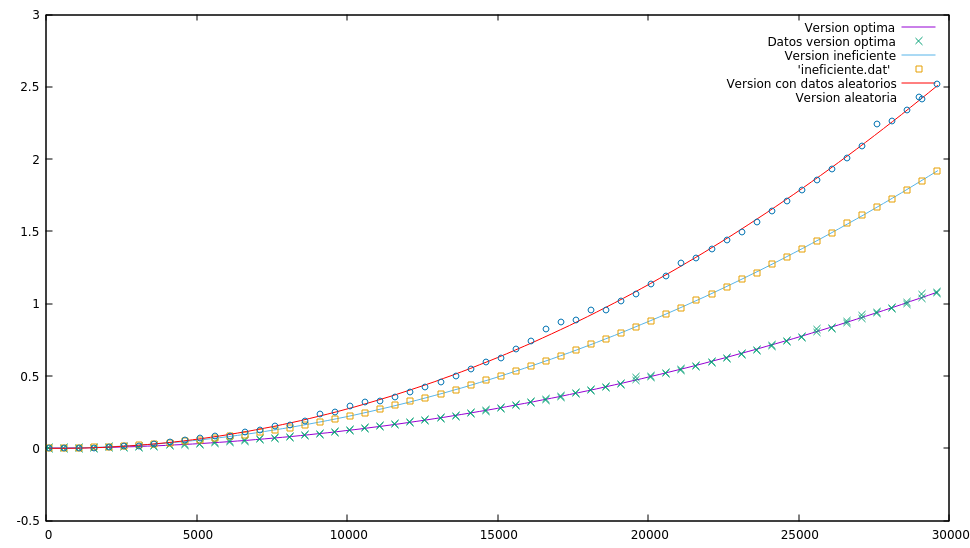
\includegraphics[width=0.8\textwidth]{ejer4/comparacion.png}
  \end{figure}

  \begin{flushleft}
    Por algún motivo, la gráfica cuando la función toma valores
    aleatorios está por encima de cuando toma valores en el caso más
    desfavorable. No se ha debido a un error en los vectores ya que
    estos se generan correctamente.
  \end{flushleft}
